\starredchapter{ANNEXE~\thechapter. ANALYSES DE SENSIBILITÉ}\label{app:sensitivity}

\appsection{Sélectivité de taille}

Nous avons tenu compte de la sélectivité de taille des ERSN en excluant les échantillons de la pêche récréative qui étaient plus petits que 75 cm de longueur à la fourche (>70\,\% des échantillons de régime alimentaire étaient estimés être supérieurs à cette taille) et en rajustant le modèle présenté dans le texte principal (Équation \ref{eq:comp_eq}). Notez que la simulation de composition de taille présentée dans le texte principal teste explicitement la sélectivité de taille. L'analyse présentée ici n'a été utilisée que pour évaluer l'interaction entre la taille et la sélectivité du stock.

Nous avons généré des prédictions (effets marginaux) de la composition saisonnière du stock à travers les strates et avons comparé qualitativement ces prédictions aux prédictions du modèle du texte principal. Nous avons également évalué l'effet de l'analyse de sensibilité sur la simulation de sélectivité du stock, en utilisant un modèle ajusté uniquement aux échantillons collectés de poissons plus grands que 75 cm de longueur à la fourche pour générer des vecteurs alternatifs de composition moyenne du stock ($\hat{\pi_{s_{size}}}$). 

Nous notons que cette analyse de sensibilité n'est pas une évaluation compréhensive du biais d'échantillonnage. Par exemple, le comportement de la flotte récréative a été impacté par une gamme de mesures de gestion qui changent saisonnièrement, spatialement et entre les années \citep{dobsonTechnicalReviewManagement2020, dfoPacificRegionFinal2023}. De même, les restes de proies peuvent être plus susceptibles d'être collectés de stocks de saumon chinook ayant des comportements particuliers. Bien qu'il n'ait pas été possible de tenir compte statistiquement de ces facteurs de confusion, nous explorons leurs impacts potentiels dans la Discussion du texte principal. 

Généralement, les motifs saisonniers dans la composition du stock étaient similaires, peu importe si les modèles étaient ajustés au jeu de données complet (texte principal) ou à un jeu contraint aux grands individus seulement. Cependant, il y avait des différences subtiles pour des stocks, des strates et des périodes spécifiques. Par exemple, les stocks «\,Autre\,», Puget Sound et ECVI/SOMN étaient relativement moins abondants dans des strates spécifiques lorsque les petits individus étaient exclus (Figures \ref{fig:comb-pred-stock1}, \ref{fig:comb-pred-stock2}). Inversement, les stocks du fleuve Fraser, excluant les individus Spring $4_2$, étaient typiquement plus abondants lorsque les petits individus étaient exclus (Figure \ref{fig:comb-pred-stock2}). 

\begin{figure}[H]
    \centering
    \pdftooltip{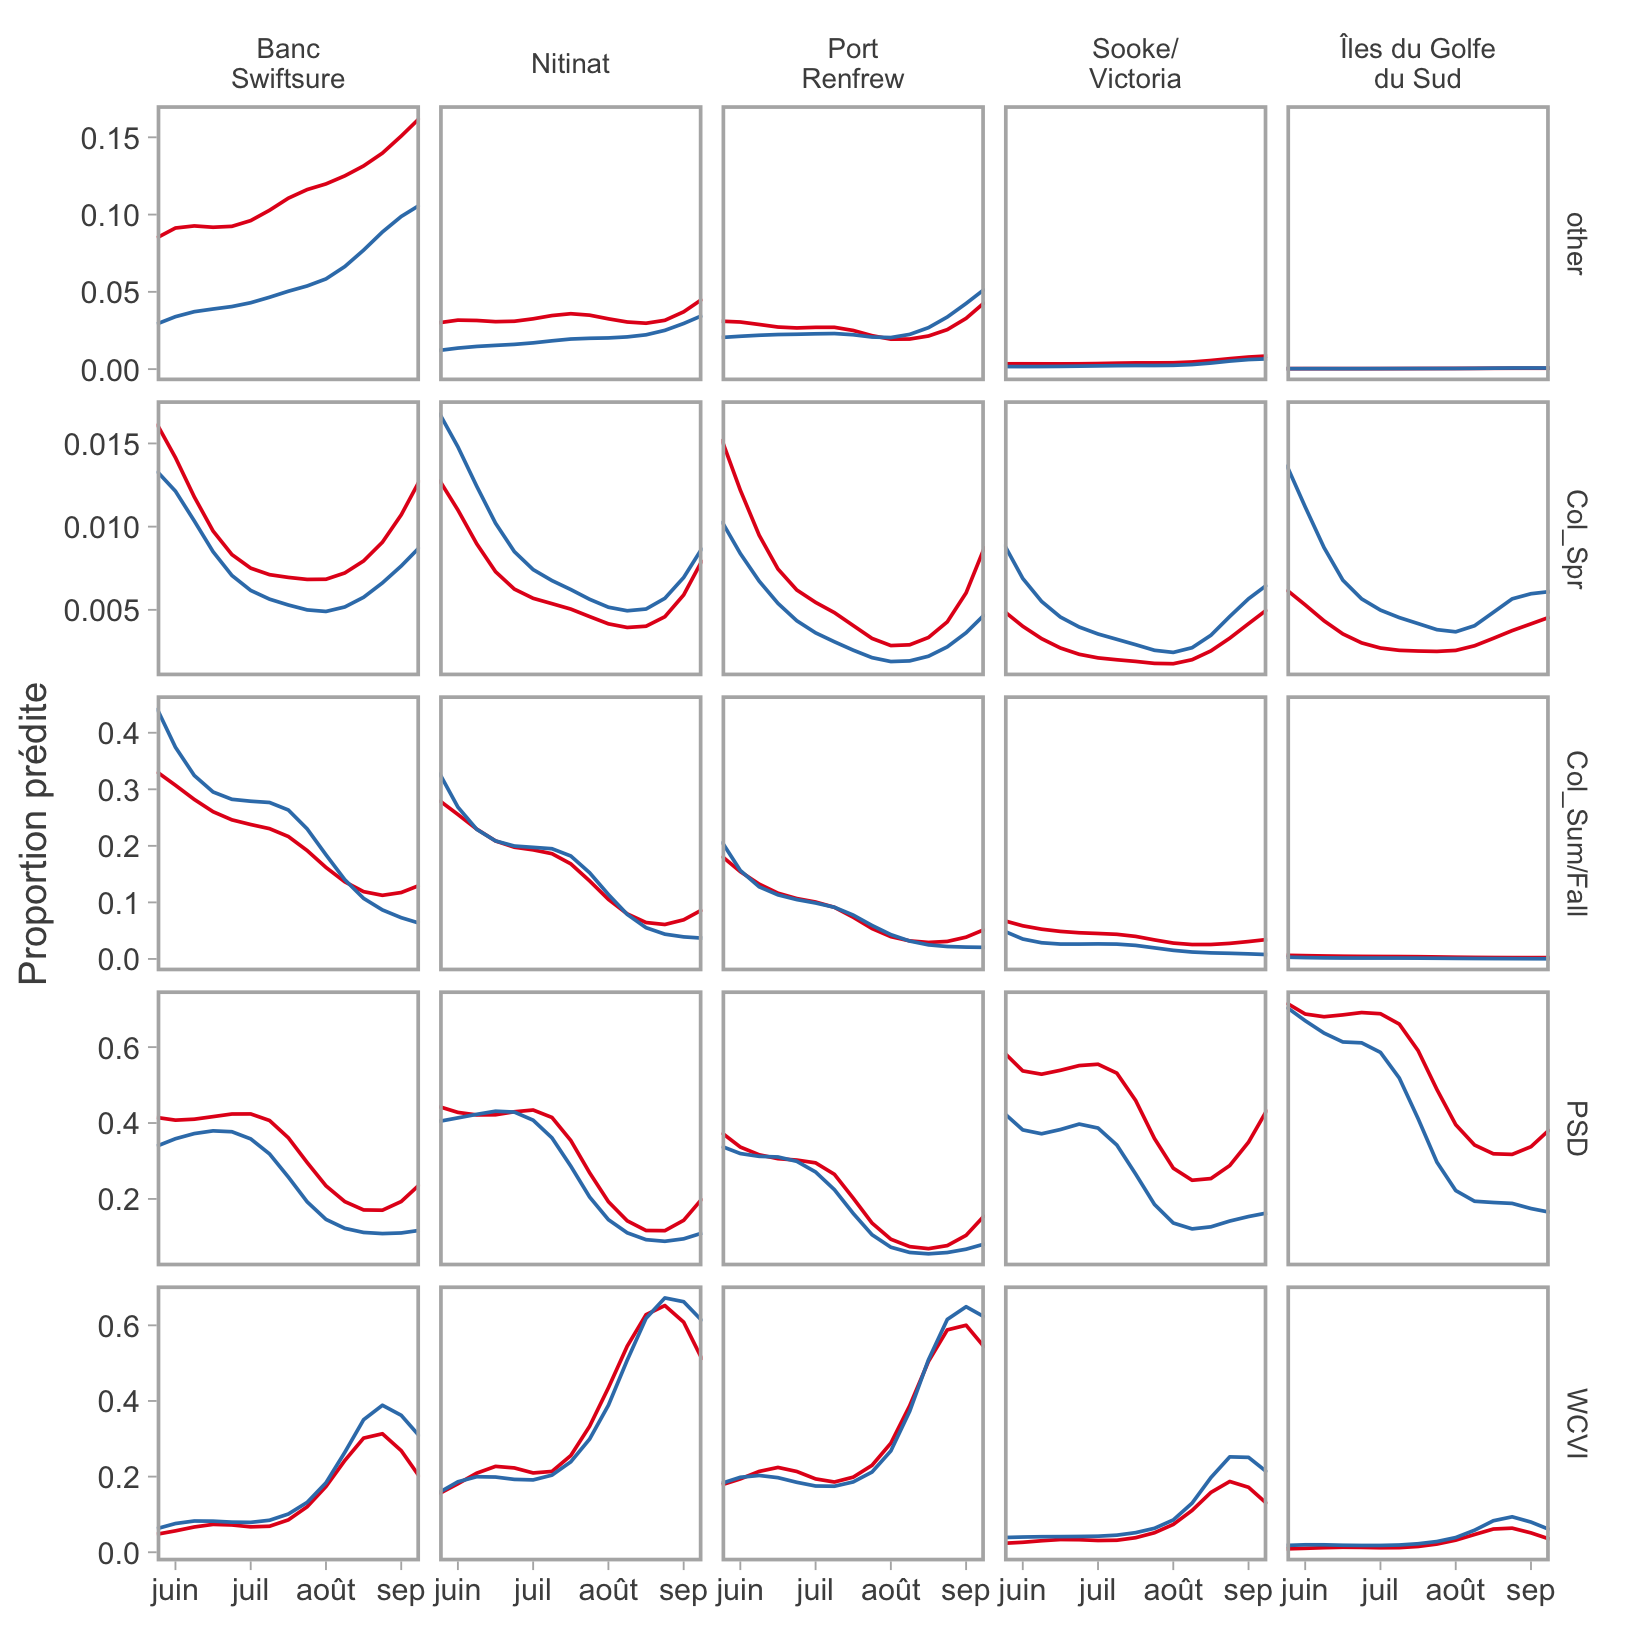
\includegraphics[width=5in]{figs/supp_figs/model_comp_stock1.png}}{Figure \ref{fig:comb-pred-stock1}}
    \caption{Prédictions saisonnières de l'abondance spécifique au stock pour les stocks autre, Columbia Spring, Columbia Summer/Fall, Puget Sound et côte ouest de l'île de Vancouver. Les prédictions sont basées sur le modèle standard présenté dans le texte principal (rouge), ainsi qu'un modèle ajusté uniquement aux données d'individus plus grands que 75 cm (bleu). Les prédictions représentent les estimations moyennes et les intervalles de confiance ne sont pas montrés pour améliorer la lisibilité. Notez les différences d'échelle de l'axe des y entre les stocks.}
    \label{fig:comb-pred-stock1}
\end{figure}

\begin{figure}[H]
    \centering
    \pdftooltip{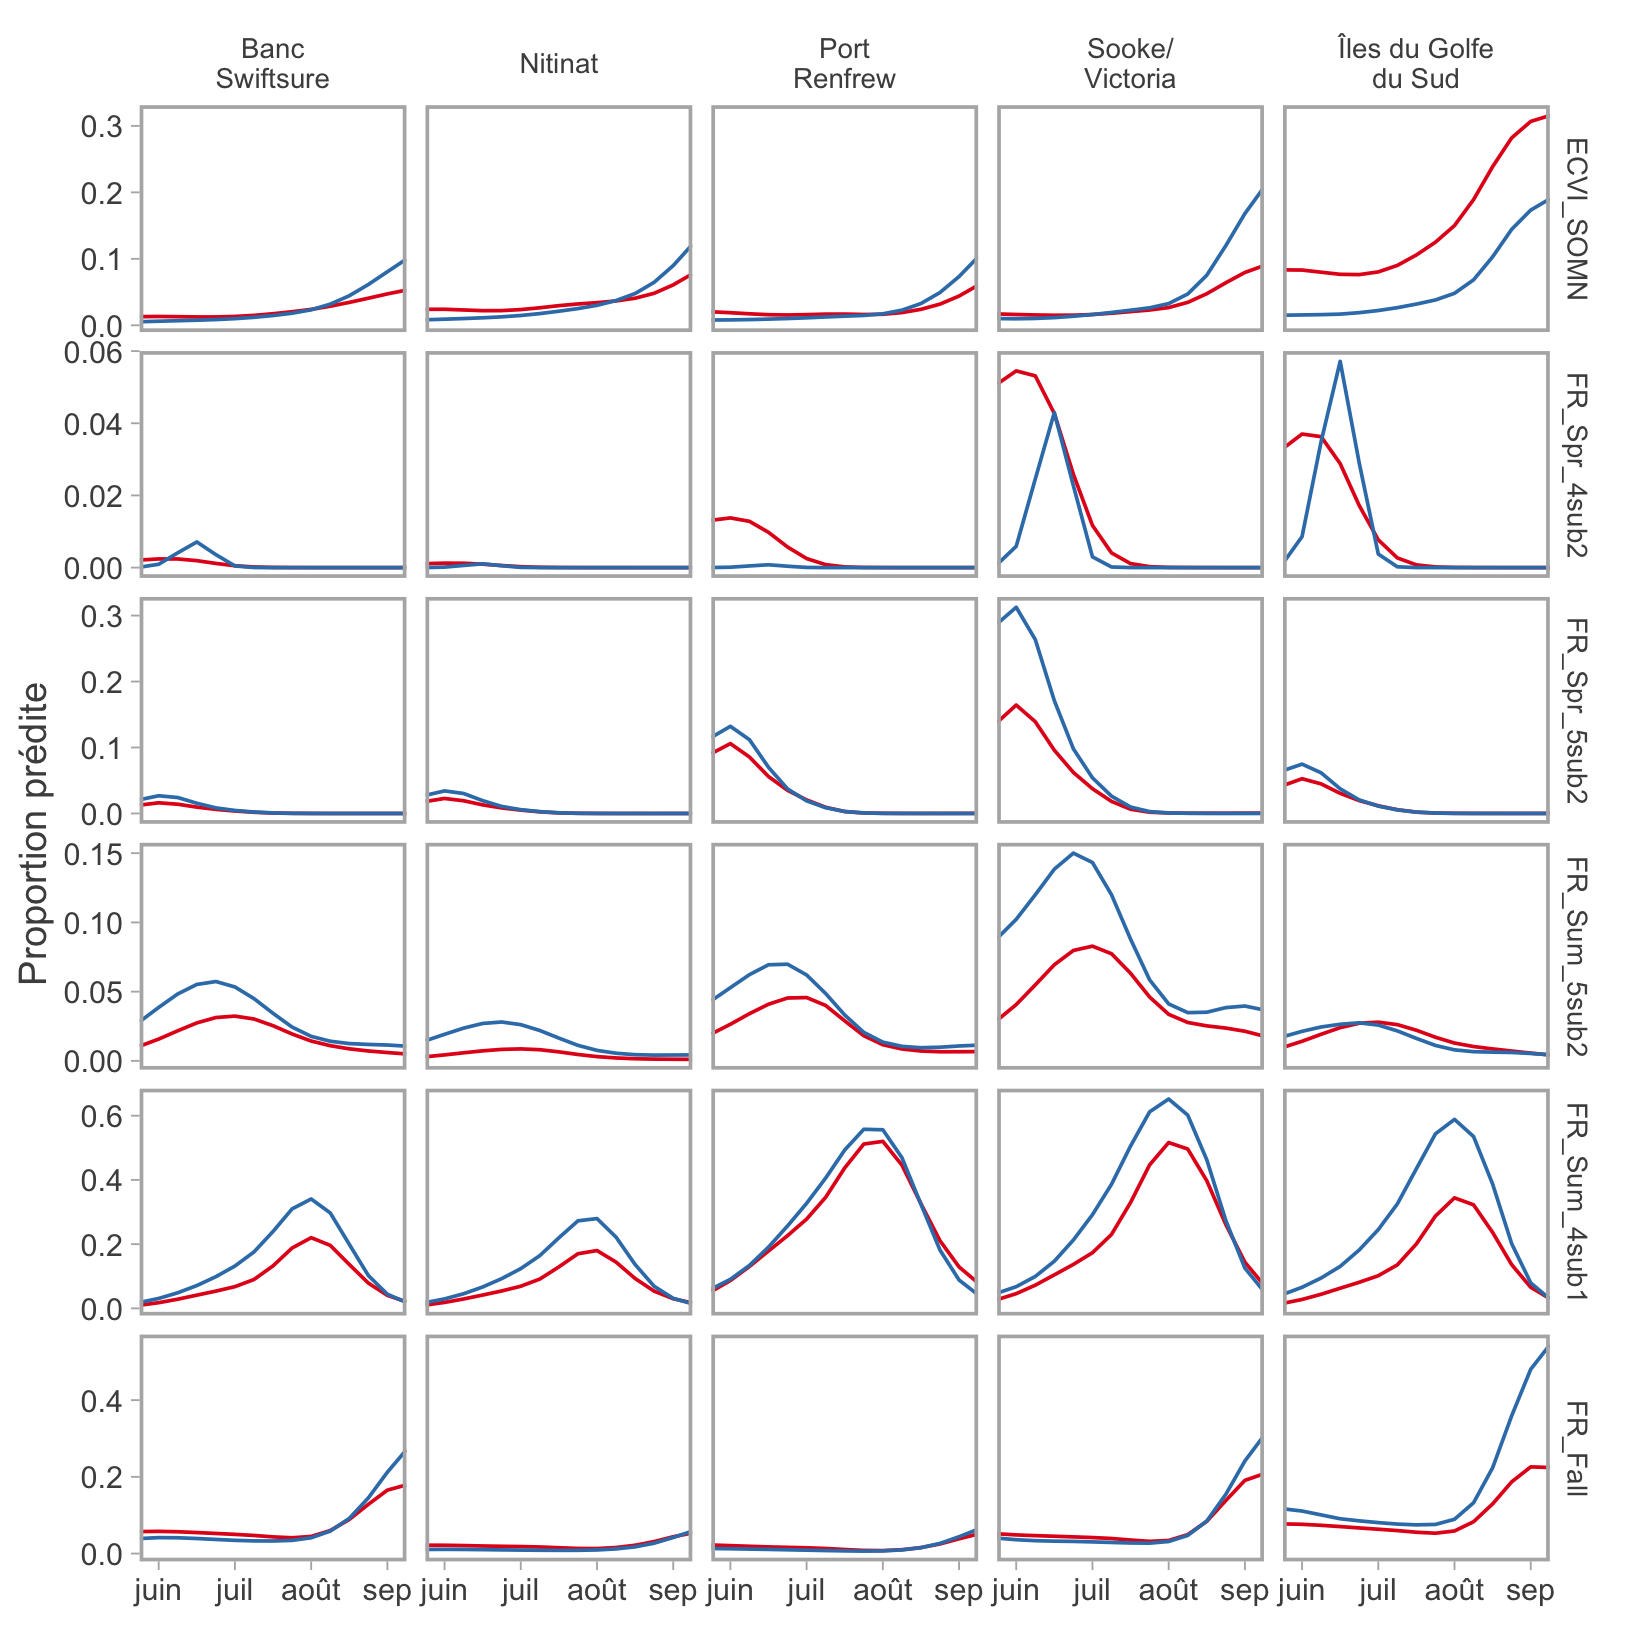
\includegraphics[width=5in]{figs/supp_figs/model_comp_stock2.png}}{Figure \ref{fig:comb-pred-stock2}}
    \caption{Prédictions saisonnières de l'abondance spécifique au stock pour les stocks ECVI/SOMN et du fleuve Fraser. Les prédictions sont basées sur le modèle standard présenté dans le texte principal (rouge), ainsi qu'un modèle ajusté uniquement aux données d'individus plus grands que 75 cm (bleu). Les prédictions représentent les estimations moyennes et les intervalles de confiance ne sont pas montrés pour améliorer la lisibilité. Notez les différences d'échelle de l'axe des y entre les stocks.}
    \label{fig:comb-pred-stock2}
\end{figure}

La composition simulée du modèle du scénario des grands individus était légèrement plus cohérente avec les restes de proies observés (Figure \ref{fig:comb-sel-stock}). Par exemple, la différence dans l'abondance proportionnelle des poissons de Puget Sound a diminué. Ces motifs suggèrent que la sélectivité de taille par les ERSN a contribué aux différences dans la composition du stock entre les prédictions du modèle et les échantillons observés. Néanmoins, ces différences étaient modestes et il y avait encore des preuves solides de surreprésentation pour les stocks Fraser River Summer $4_1$, Summer $5_2$ et Spring $5_2$, ainsi que de sous-représentation des stocks WCVI, Columbia River Summer/Fall et «\,Autre\,» (Figure \ref{fig:comb-sel-stock}). 

\begin{figure}[H]
    \centering
    \pdftooltip{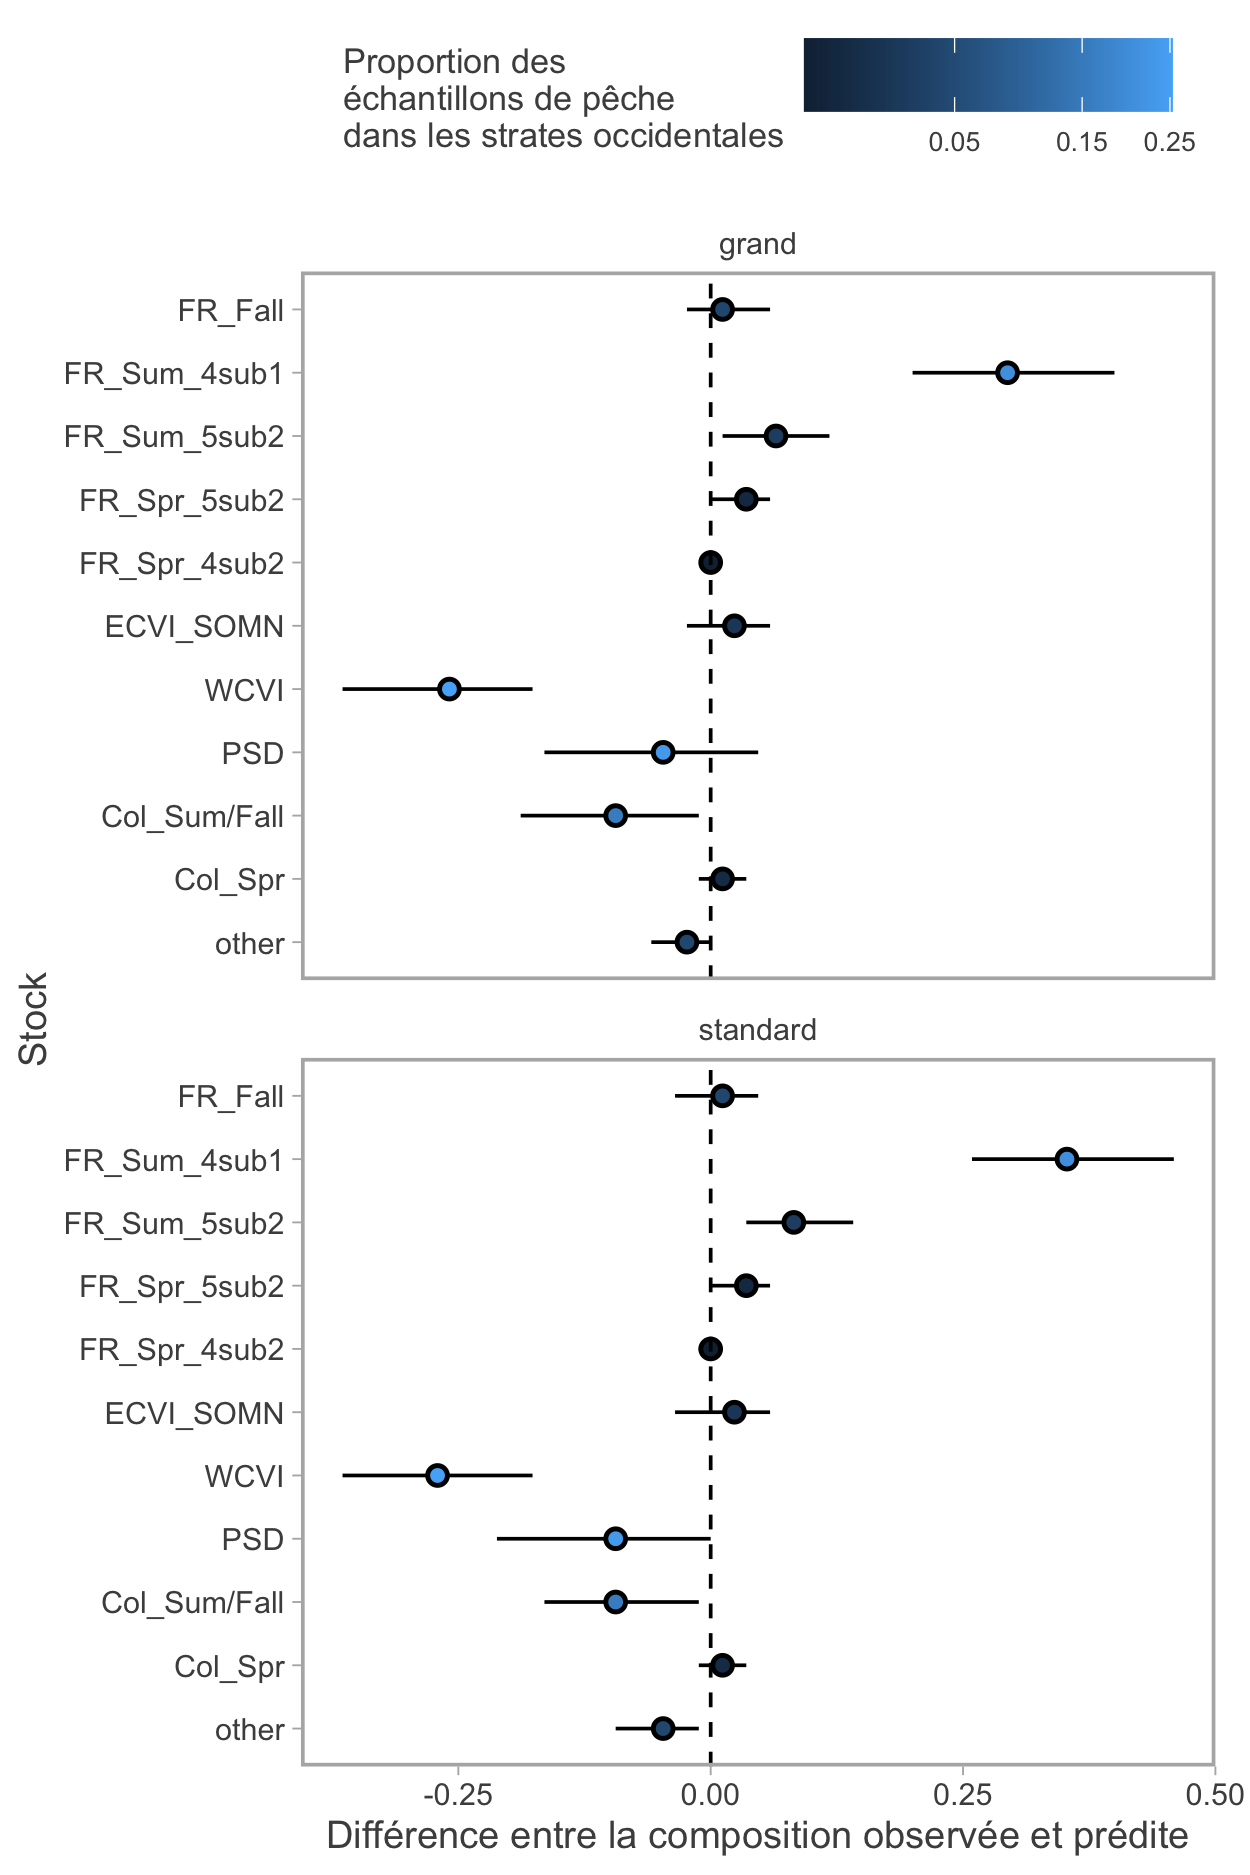
\includegraphics[width=5in]{figs/supp_figs/selectivity_bean_stock_comp.png}}{Figure \ref{fig:comb-sel-stock}}
    \caption{Différences entre la contribution observée et prédite par le modèle de chaque stock aux restes de proies des ERSN en utilisant le modèle standard présenté dans le texte principal (haut) et un modèle ajusté aux données excluant les individus plus petits que 75 cm de longueur à la fourche (bas). Les valeurs positives (négatives) indiquent qu'un stock donné a été observé plus (moins) fréquemment dans les restes de proies des ERSN que prédit par le modèle dépendant de la pêcherie. Les points représentent les médianes et les moustaches représentent les intervalles du 95e percentile parmi 500 simulations Monte Carlo. Les points plus lumineux (plus sombres) représentent les stocks qui étaient plus (moins) communs dans les échantillons de la pêche récréative des moments et strates coïncidant avec les restes de proies des ERSN.}
    \label{fig:comb-sel-stock}
\end{figure}

\appsection{Interventions de gestion}

Pour évaluer l'impact des interventions de gestion sur la sélectivité, nous avons retiré de la simulation les échantillons de proies qui ont été collectés pendant les moments et emplacements où les pêcheries coïncidentes étaient fermées ou impactées par les limites de taille maximales. 11 échantillons de proies ont été retirés de l'analyse de sélectivité du stock et huit ont été retirés de l'analyse de sélectivité de taille. Nous avons ensuite répété l'analyse de simulation et comparé les résultats aux résultats originaux présentés dans le texte principal.

Les estimations de sélectivité du stock (Figure \ref{fig:comb-sel-stock2}) et de taille (Figure \ref{fig:comb-sel-size2}) étaient qualitativement inchangées lorsqu'un ensemble plus conservateur de proies a été inclus dans la simulation. Ces résultats indiquent que la sélectivité du stock et de taille n'était pas uniquement motivée par la présence d'interventions de gestion. Cependant, il n'est pas possible de quantifier l'impact des interventions de gestion à travers la zone d'étude sur les estimations du modèle.

\begin{figure}[H]
    \centering
    \pdftooltip{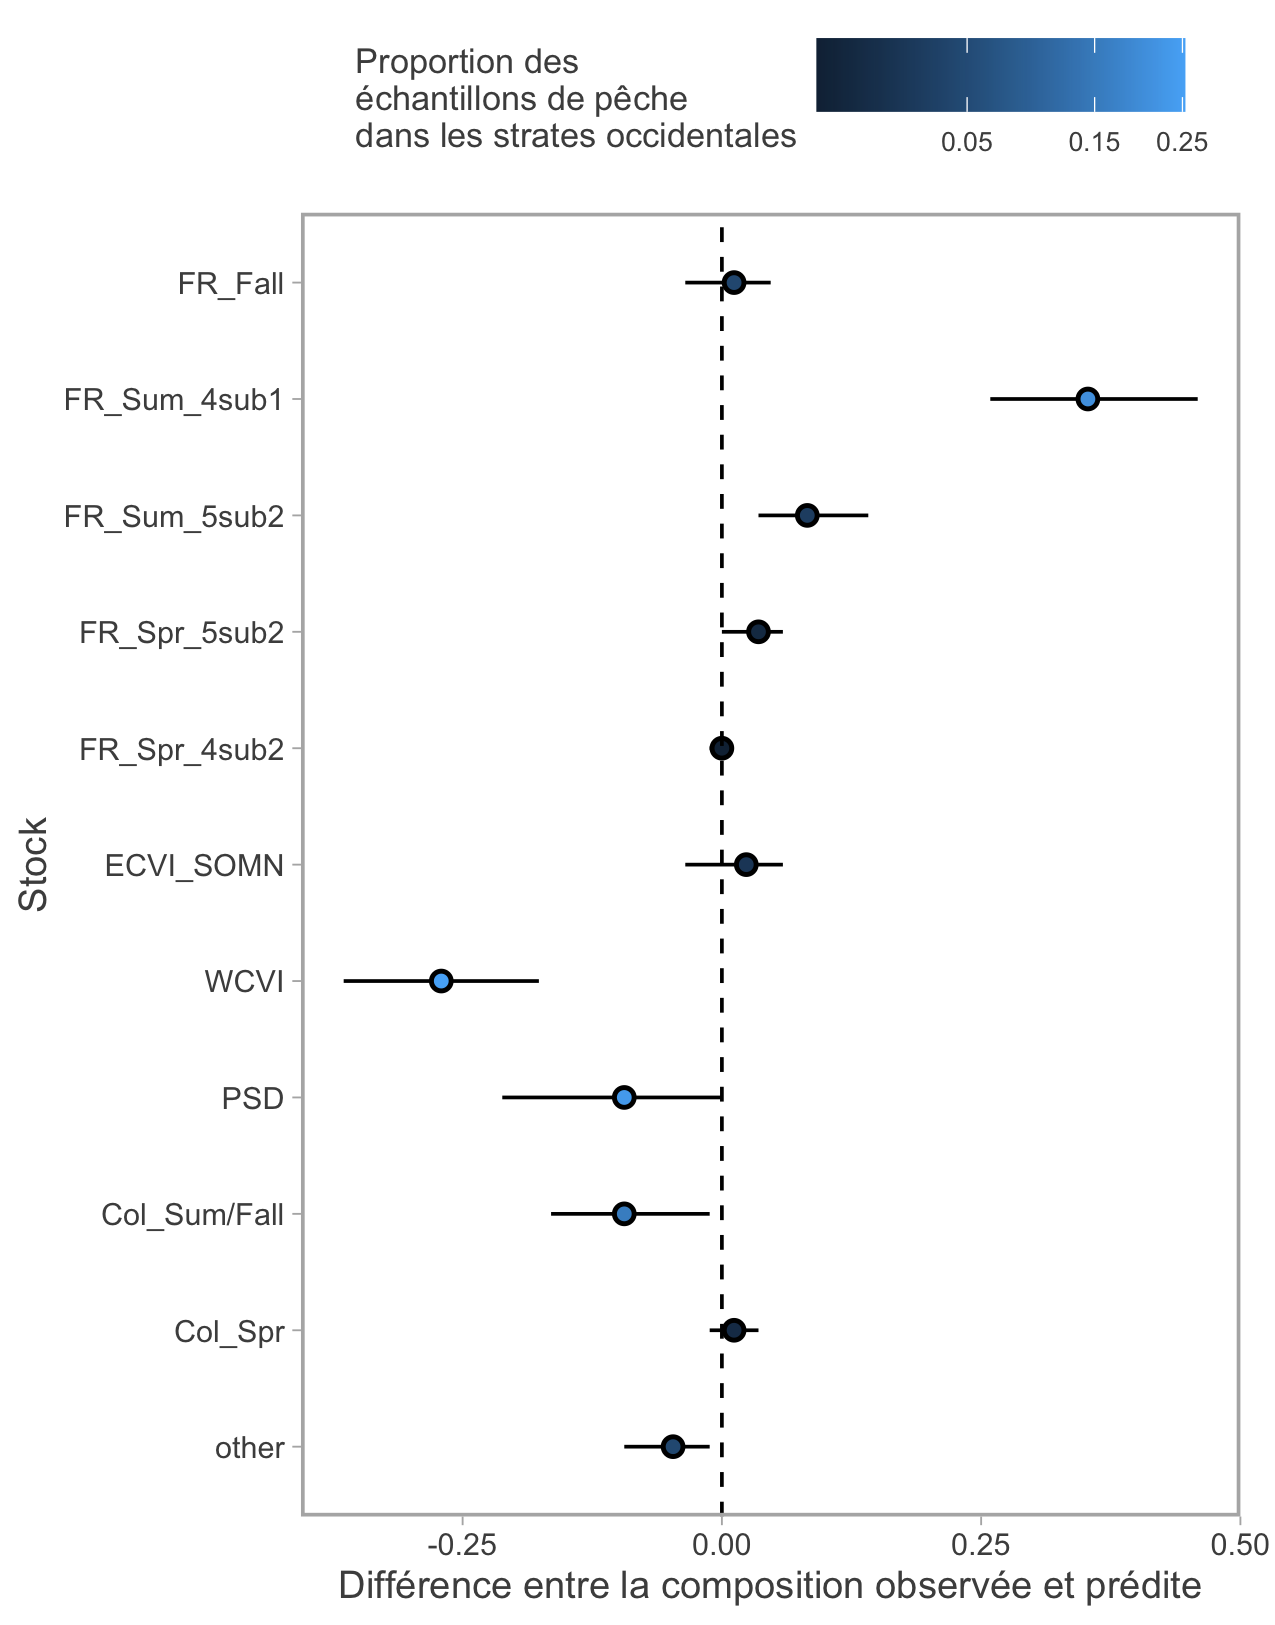
\includegraphics[width=5in]{figs/supp_figs/selectivity_bean_stock_sens.png}}{Figure \ref{fig:comb-sel-stock2}}
    \caption{Différences entre la contribution observée et prédite par le modèle de chaque stock aux restes de proies des ERSN en utilisant le jeu de données complet des restes de proies présenté dans le texte principal (haut) et les restes de proies qui ont exclu les échantillons collectés dans les moments et emplacements où les interventions de gestion étaient en place (bas). Les valeurs positives (négatives) indiquent qu'un stock donné a été observé plus (moins) fréquemment dans les restes de proies des ERSN que prédit par le modèle dépendant de la pêcherie. Les points représentent les médianes et les moustaches représentent les intervalles du 95e percentile parmi 500 simulations Monte Carlo. Les points plus lumineux (plus sombres) représentent les stocks qui étaient plus (moins) communs dans les échantillons de la pêche récréative des moments et strates coïncidant avec les restes de proies des ERSN.}
    \label{fig:comb-sel-stock2}
\end{figure}

\begin{figure}[H]
    \centering
    \pdftooltip{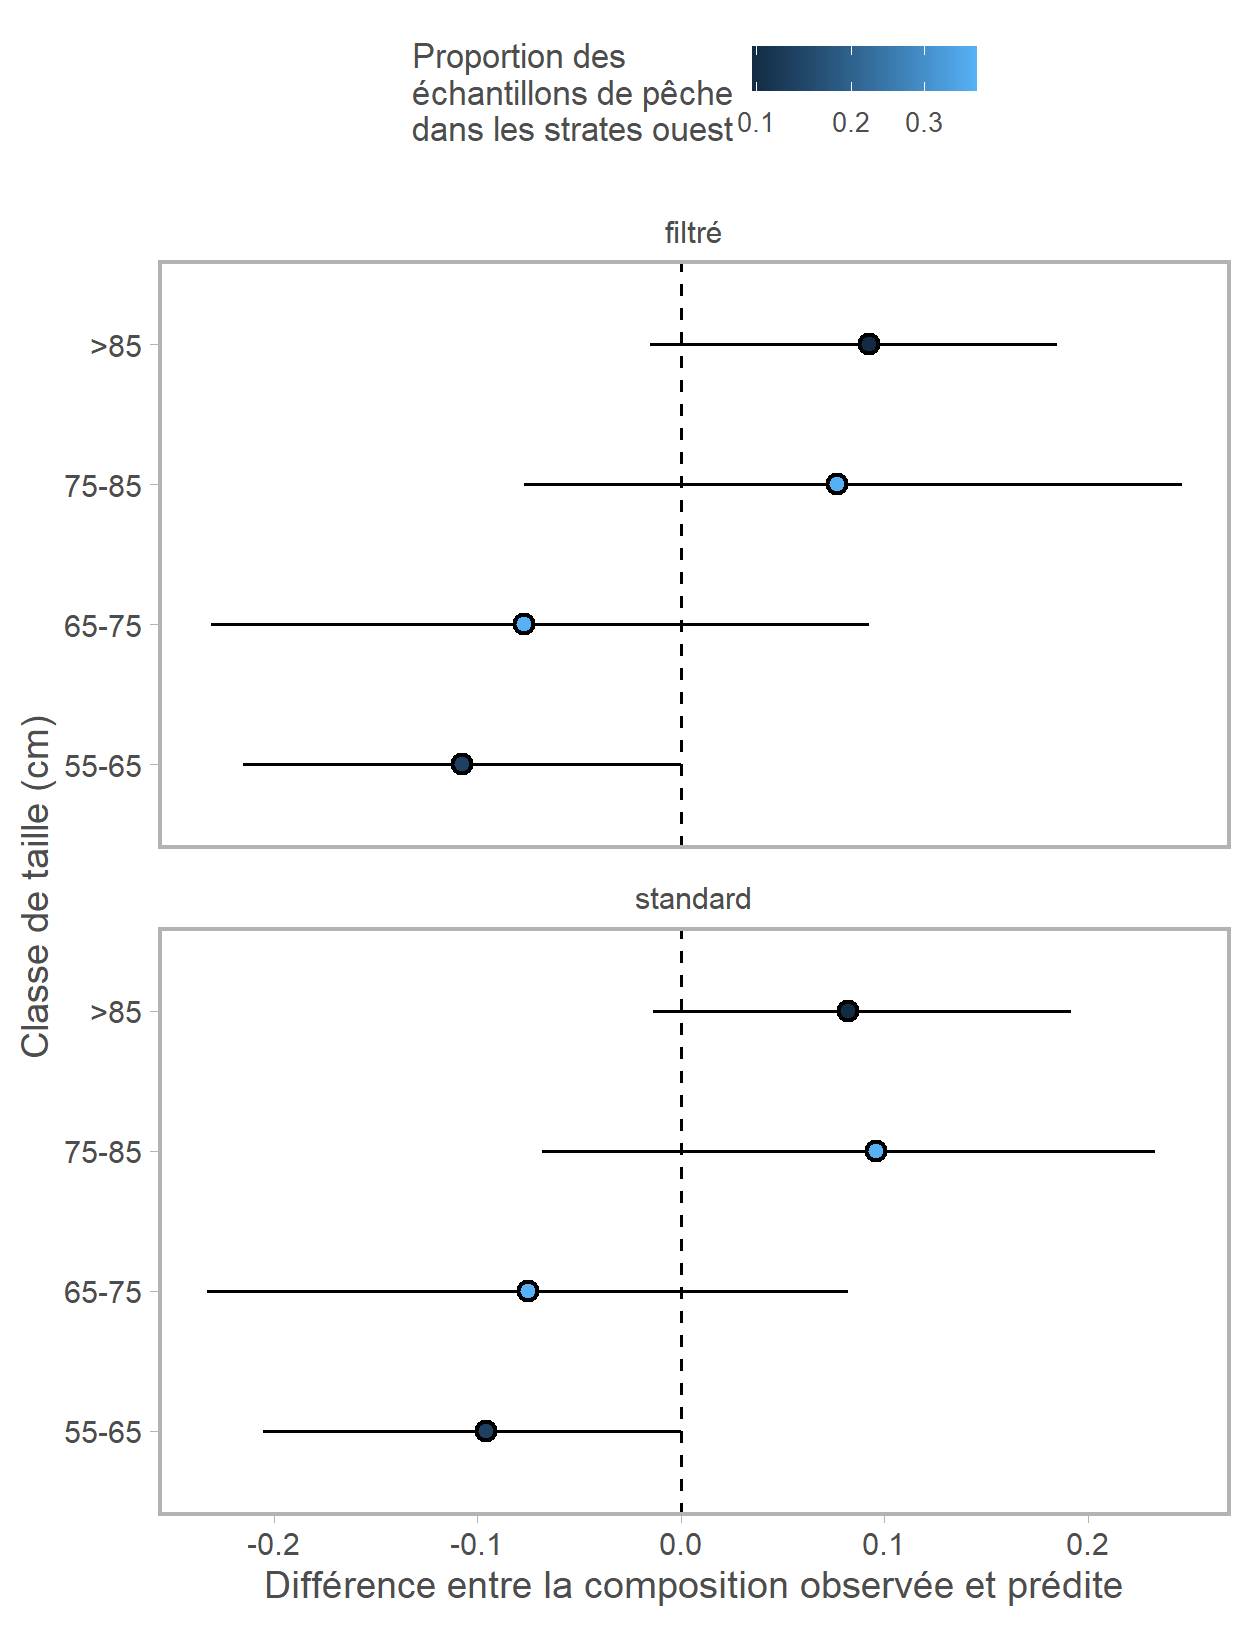
\includegraphics[width=5in]{figs/supp_figs/selectivity_bean_size_sens.png}}{Figure \ref{fig:comb-sel-size2}}
    \caption{Différences entre la contribution observée et prédite par le modèle de chaque classe de taille aux restes de proies des ERSN en utilisant le jeu de données complet des restes de proies présenté dans le texte principal (haut) et les restes de proies qui ont exclu les échantillons collectés dans les moments et emplacements où les interventions de gestion étaient en place (bas). Les valeurs positives (négatives) indiquent qu'une classe de taille donnée a été observée plus (moins) fréquemment dans les restes de proies des ERSN que prédit par le modèle dépendant de la pêcherie. Les points représentent les médianes et les moustaches représentent les intervalles du 95e percentile parmi 500 simulations Monte Carlo. Les points plus lumineux (plus sombres) représentent les classes de taille qui étaient plus (moins) communes dans les échantillons de la pêche récréative des moments et strates coïncidant avec les restes de proies des ERSN.}
    \label{fig:comb-sel-size2}
\end{figure}

